%!TEX TS-program = xelatex
%!TEX encoding = UTF-8 Unicode

%%
%% 使用 njuthesis 文档类生成南京大学本科生毕业论文的示例文档
%% 
%%

%% 
%% 南京大学本科学位论文模板

%% 如需Adobe字体请用
%% 如果字体不全使用Adobe选项可能会报错
%\documentclass[adobefonts]{njuthesis}
%% MacOS系统请用
\documentclass[macfonts]{njuthesis}
%% Windows系统请用
%\documentclass[winfonts]{njuthesis}
%% Linux系统请用
%\documentclass[linuxfonts]{njuthesis}

\usepackage[labelfont=bf]{caption}
\usepackage{mathptmx,multirow}
\usepackage{wrapfig}
\newtheorem{thm}{定理}[chapter]
\newtheorem{defn}[thm]{定义}
\newtheorem{rem}[thm]{注释}
\newtheorem{lem}[thm]{引理}
\newtheorem{cor}[thm]{推论}
\newtheorem{asp}[thm]{假设}
\newtheorem*{Proof}{证明}




% 行距 1.5
% laTex默认1.2行距,所以1.2/1.5 = 1.25
\linespread{1.25}
% \setstretch{1.5}
% %%%%%%%%%%%%%%%%%%%%%%%%%%%%%%%%%%%%%%%%%%%%%%%%%%%%%%%%%%%%%%%%%%%%%%%%%%%%%%%
% 设置论文的中文封面
% 论文标题
\title{非光滑复合优化与拓展流形采样算法}

% 论文作者姓名
\author{马宇恒}
% 论文作者学号
\studentid{171240510}
% 导师姓名职称
\supervisor{顾国勇}
% 导师职称
\supervisortitle{副教授}
% 论文作者院系
\department{匡亚明学院}
% 论文作者专业方向
\major{理强(统计学)}
% 论文作者的年级
\grade{2017级}
% 论文提交日期,需设置年、月、日。此属性可选,默认值为最后一次编译时的日期,精确到日。
\submitdate{2021年6月8日}

%%%%%%%%%%%%%%%%%%%%%%%%%%%%%%%%%%%%%%%%%%%%%%%%%%%%%%%%%%%%%%%%%%%%%%%%%%%%%%%
% 设置论文的英文封面

% 论文的英文标题
\englishtitle{Nonsmooth Nonconvex Compositions Optimization and Generalized Manifold Sampling}
% 论文作者姓名的拼音
\englishauthor{Yuheng Ma}
% 导师姓名职称的英文
\englishsupervisor{Guoyong Gu}
% 论文作者所在院系的英文名称
\englishdepartment{Kuang Yaming Honors School}
% 论文作者所在学校或机构的英文名称。此属性可选,默认值为``Nanjing University''。
\englishinstitute{Nanjing University}
% 论文完成日期的英文形式,默认最后一次编译的时间
\englishdate{June 8, 2021}
% 专业
\englishinstitute{DII(Statistics)}
%%%%%%%%%%%%%%%%%%%%%%%%%%%%%%%%%%%%%%%%%%%%%%%%%%%%%%%%%%%%%%%%%%%%%%%%%%%%%%%
% 设置论文的页眉页脚
\usepackage{fancyhdr}
\pagestyle{fancy}
%\lhead{\bfseries 141180092 }
\chead{非光滑复合优化与拓展流形采样算法}
\rhead{马宇恒}
%\lfoot{From: K. Grant}
%\cfoot{To: Dean A. Smith}
%\rfoot{\thepage}
\renewcommand{\headrulewidth}{0.4pt}
%\renewcommand{\footrulewidth}{0.4pt}
%%%%%%%%%%%%%%%%%%%%%%%%%%%%%%%%%%%%%%%%%%%%%%%%%%%%%%%%%%%%%%%%%%%%%%%%%%%%%%%
\begin{document}

% 制作中文封面
\maketitle
% 制作英文封面
\makeenglishtitle
% 毕业论文过程管理四页表
\controlpage 
%可以将word文件交给老师签字后扫描转成pdf,然后命名为controlpage.pdf

% 论文的中文摘要
\begin{abstract}

非光滑无导数优化是数值优化领域里富有前景但充满挑战的方向。流形采样算法是一类基于局部模型的无导数优化模型,其可以优化函数$f=h\circ F$,其中$h$为非凸非光滑函数,$F$为光滑映射,但其雅可比矩阵很难获得。算法通过在$x$附近随机采样,建立$F$在$x$附近的模型,结合$h$的信息,得到下降点,从而生成收敛到$f$的Clark稳定点的序列。我们拓展已有的流形采样算法至更加广泛的形式,允许f的形式为$f=h\circ F+\phi$,其中$\phi$为光滑函数,使得算法能够对一类常用形式的非光滑、非凸复合函数,即机器学习中常用的损失+惩罚形式的目标函数,进行无导数优化。在证明了算法收敛性的同时,我们完成了丰富的数值试验,在标准测试集上检验了算法,并经验的讨论了实验结果。最后,我们采用该算法训练浅层神经网络,展示了算法的有效性。

% 同时应该注意到,空白页是故意留白,以便章节开头能够出现在偶数页。
% 中文关键词。关键词之间用中文全角分号隔开,末尾无标点符号。
\keywords{非光滑优化;无导数优化;复合优化;流形采样}
\end{abstract}

%%%%%%%%%%%%%%%%%%%%%%%%%%%%%%%%%%%%%%%%%%%%%%%%%%%%%%%%%%%%%%%%%%%%%%%%%%%%%%%
% 论文的英文摘要
\begin{englishabstract}
Non-smooth derivative free optimization method is a challenging but promising topic in optimization. Manifold sampling is a type of model based derivative free algorithm that optimize the composition $f=h\circ F$, where $h$ is a non-smooth non-convex function, $F$ is a smooth map without inexpensive Jacobian. Algorithm build local model of $F$ around by sampling, which is combined with information of $h$ to acquire decrease point. It generates a sequence converging to Clark stationary point of f. We modified manifold sampling algorithm to a more general case, allowing $f=h\circ F+\phi$, such that it can optimize non-smooth, non-convex compositions in a derivative free way. As convergence guarantee for the generalized algorithm provided, we also implement various numerical experiments and discussed results empirically. Meanwhile, we train neural network using manifold sampling, illustrating its power.
% 英文关键词。关键词之间用英文半角逗号隔开,末尾无符号。
\englishkeywords{Non-smooth Optimization, Derivative Free Optimization, Composite Optimization, Manifold Sampling}
\end{englishabstract}

%%%%%%%%%%%%%%%%%%%%%%%%%%%%%%%%%%%%%%%%%%%%%%%%%%%%%%%%%%%%%%%%%%%%%%%%%%%%%%%
% 论文的前言,应放在目录之前,中英文摘要之后
%
%\begin{preface}
%
%在过去的40年中,手写中文文本领域识别(HCTR)取得了很大的进展[1,2]。
%
%\vspace{1cm}
%\begin{flushright}
%饶安逸\\
%2018年5月15日于南大仙林
%\end{flushright}
%
%\end{preface}

%%%%%%%%%%%%%%%%%%%%%%%%%%%%%%%%%%%%%%%%%%%%%%%%%%%%%%%%%%%%%%%%%%%%%%%%%%%%%%%
% 生成论文目录
\tableofcontents

%%%%%%%%%%%%%%%%%%%%%%%%%%%%%%%%%%%%%%%%%%%%%%%%%%%%%%%%%%%%%%%%%%%%%%%%%%%%%%%
% 生成插图清单。如无需插图清单则可注释掉下述语句。
%\listoffigures

%%%%%%%%%%%%%%%%%%%%%%%%%%%%%%%%%%%%%%%%%%%%%%%%%%%%%%%%%%%%%%%%%%%%%%%%%%%%%%%
% 生成附表清单。如无需附表清单则可注释掉下述语句。
%\listoftables

%%%%%%%%%%%%%%%%%%%%%%%%%%%%%%%%%%%%%%%%%%%%%%%%%%%%%%%%%%%%%%%%%%%%%%%%%%%%%%%
% 开始正文部分
\mainmatter

%%%%%%%%%%%%%%%%%%%%%%%%%%%%%%%%%%%%%%%%%%%%%%%%%%%%%%%%%%%%%%%%%%%%%%%%%%%%%%%
% 学位论文的正文应以《绪论》作为第一章
\chapter{绪论}\label{chapter_introduction}
\section{研究背景}
无约束的复合优化是非光滑优化中一类重要的问题,其通常形式如下:
\begin{equation}
\underset{x}{\operatorname{minimize}} \~\quad f(x) \triangleq \phi(x)+h(F(x)),  \; x \in \mathbb{R}^n. 
\label{problem}
\end{equation}

其中$\phi$为光滑函数,并且在很多情形下为0 。$F: \mathbb{R}^{n} \rightarrow \mathbb{R}^{p}$为光滑函数,$h: \mathbb{R}^{p} \rightarrow \mathbb{R}$为连续但不可导,而且通常被假设为凸函数。这类问题经常伴随着优化与范数有关的损失函数。\par
%在当下最热门的深度学习中,n分类问题大多使用的Softmax层\cite{PRML}作为最终输出,返回一个代表各类别概率的n维向量$f(x)\in [0,1]^n$。神经网络参数的优化就是要优化$||y-f()||$亦即最小化$\Sigma||y_i-f(x_i)||$。
在机器学习中,添加惩罚项能够促使参数朝着理想的方向靠近,如减小参数尺度的岭回归和神经网络中的权重衰减使用了$L^2$惩罚,Lasso回归\cite{Lasso}是$L^1$惩罚的结果,ElasticNet惩罚\cite{ElasticNet}则是二者的结合,还有缩减秩的$L^0$范数。当范数算子为非光滑,如$L^1$或$L^{\infty}$范数\cite{NonlinearEqLInfty}时,优化问题即为复合优化。
\par
复合优化在控制、信号处理领域有很多实际应用\cite{CharalambousC},如分散式控制系统\cite{distributedcontrol}和低复杂性建模\cite{lowcomplexity}。John Duchi和Ruan Feng\cite{phaseretrieval}考虑在相位恢复问题中应用复合优化,考虑真实信号$x^*\in \mathbb{R}^n$和量测向量$(a_1,\cdots,a_n)$,观察信号为$b_i=\phi(<a_i,x^*>)+\epsilon_i,\;i=1,\cdots,n$,其中$\phi$为非线性函数。则$x^*$的估计可以通过$min_x \frac{1}{n} \sum_{i=1}^{n}\left(\phi\left(\left\langle a_{i}, x\right\rangle\right)-b_{i}\right)^{2}$得到。然而实际过程中观察到的往往是$b_{i}=\left\langle a_{i}, x^{\star}\right\rangle^{2}$,所以需要优化$\frac{1}{n} \sum_{i=1}^{n}\left|\left\langle a_{i}, x\right\rangle^{2}-b_{i}\right|$,从而成为复合优化问题。

许多经典优化问题同样可以转化为复合优化。考虑一组非线性方程$F_i(x)=0,\;i=1,\cdots,n$,方程的求解等价于优化$||F(x)||=||(F_1,\cdots,F_n)||$,$||\cdot||$为任意的范数算子\cite{NonlinearEqLp}。当算子为非光滑,问题即为复合优化。寻找非线性系统的可行点也可以视为复合优化问题。考虑一系列非线性不等式约束$F_i(x)\leq 0,\;i=1,\cdots,n$,则可行点的寻找等价于求解$min\;\Sigma ||F^+_i(x)||$,其中$F^+_i(x)=max(F_i(x),0)$。

\section{相关工作}
复合优化的理论最先由A. D. Ioffe \cite{IoffeAD1979}建立,并且给出了$h$为次线性的局部极小条件。而后,J. V. Burke\cite{BerkeJV1987}将$h$的限制条件放宽至凸函数。当F为局部Lipschitz且Gâteaux可微时,Jeyakumar 和 X. Q. \cite{Lagrange}给出了一阶拉格朗日必要条件和二阶充分条件。在F的导数容易取得的情况下,\cite{comp21,comp22,comp56}都给出了理论分析。
而就数值算法而言,在直接使用梯度的算法失效后,近端梯度下降\cite{proximal,accproximal}成为了很好的替代品,即便它们需要非光滑项关于变量可分离这一很强的假设。通过将光滑项与非光滑项的变量分离并添加等式约束,将问题转化为约束优化,交替方向乘子法(ADMM)\cite{ADMM}等一系列方法便可以使用。此时问题被分解为光滑或者容易求解的非光滑子问题,便于分布式计算。但是在$\phi$非凸的情形下,这些方法均没有很好的收敛性保障。而乘子法(Methhod of Multipliers)\cite{MM}虽然可以提供很好的收敛保障,但由于其需要针对所有变量优化增广拉格朗日函数,计算速度被大大限制。Dhingra和Khong\cite{proximalauglag}通过在非光滑项进行最小化找到相应流型,再将增广拉格朗日映射至该流型,找到了光滑的近端增广拉格朗日函数,使得问题同时具有分布式算法、明确的参数调整方法和凸情形下的理论收敛性。束方法\cite{bundle,bundle2,bundle3}是非光滑优化中常用的方法,并且在非凸情形下也有很好的表现,当条件放宽至无法得到F的导数(Derivative-free)时依然可以使用\cite{bundlefree1,bundlefree2}。
\par
然而,正如很多文章中要求h为某个范数,如$L^2$范数\cite{comp55}、$L^{\infty}$范数\cite{comp44,comp56},几乎所有已知的算法都要求h为凸函数。Larson, Menickellly和Wild\cite{manifoldl1}提出了流型采样的方法(Manifold Sampling),在置信域方法的框架下,通过$F(x)$在附近的流型上的估计和h的Clarke方向导数来估计f(x)。虽然文章采用了$L^{1}$范数作为分析对象,但其理论与实现均不依赖h的凸性。同时,当F的导数难以取得时,流型采样方法仍然可以使用,并且相比梯度采样方法\cite{grasam1,grasam2}有非随机性的优势。Khan, Larson和Wild\cite{manifoldpiecewiselinear}拓展了这一工作,使得h可以是任意的分段线性函数。Larson, Menickelly和Zhou\cite{manifold}最近将结果拓展至$h$为任意连续函数并且其Clarke次导数可计算的情形,同时要求$\phi$为0。这是目前唯一允许$h$为任意连续函数且无需$F$一阶信息的工作。
\section{本文主要工作}
在本课题中,我们将Larson, Menickelly和Zhou的工作\cite{manifold}扩展到的$\phi$是一个光滑函数的情况。具体工作包括:



\begin{enumerate}
\item 提出了在拓展情况下的算法形式。

\item 证明了该形式理论上的收敛性。

\item 实现了基于Python的流形采样软件包。
\item 在简单样例上击败了经典优化方法,在标准测试函数集上进行了算法测试,得到了良好的结果。
\item 使用了流形采样算法训练神经网络。

\end{enumerate}

\section{本文结构}
本文的各章节组织结构如下:

第一章:绪论。简要说明了非光滑非凸复合优化的研究意义与背景。并概括地描述了这篇文章的工作,总结了本文结构。
第二章:算法概述。阐述了算法思路与主要组成部分,给出后续证明所需的定义与假设。
第三章:理论保障。证明了算法在一定条件下的收敛性。
第四章:仿真实验。展示了算法在测试集上的表现。
第五章:总结与展望。

\chapter{算法概述}

\section{研究问题}

我们希望优化
$$
\underset{x}{\operatorname{minimize}} \; f(x) \triangleq \phi(x)+h(F(x)),  \; x \in \mathbb{R}^n. 
$$
其中$\phi: \mathbb{R}^n\rightarrow \mathbb{R}$是光滑并且二阶Lipschitz连续的函数。  $F: \mathbb{R}^{n} \rightarrow \mathbb{R}^{p}$ 是可微函数, $h: \mathbb{R}^{p} \rightarrow \mathbb{R}$ 是连续函数,但允许其非光滑、非凸。


\section{记号}

若不做特殊约定,所有范数均为$l^2$范数。集合$S$的闭包记为$\mathbf{cl}(S)$。集合$S$的内点集记为$\mathbf{int}(S)$. 集合$S$的凸包记为$\mathbf{co}(S)$。集合$S$关于$F$的像集记为$\mathbf{Im}(S)=:\{F(x)|x\in S\}$。球$B(x,\delta)$为闭球。
局部Lipschitz函数$f$在x点的广义克拉克导数为$$
\partial_{\mathrm{C}} f(x) \triangleq \operatorname{co}\left(\left\{\lim _{y^{j} \rightarrow x} \nabla f\left(y^{j}\right): y^{j} \in D\right\}\right)
$$
其中$D$为x的某个邻域。若$0\in\partial_Cf(x)$,则称x为f的Clark稳定点。一般我们使用k作为角标来代指变量在第k个循环里的值。

\section{定义与假设}
这一节中包含我们接下来需要用到的所有假设与定义。

\begin{defn}
对某个常数$\delta_{max}$和$R^n$中的点$x_0$,定义
$$
\mathcal{L}_{\max } \triangleq \bigcup_{x \in \mathcal{L}\left(x^{0}\right)} B \left(x ; \Delta_{\max }\right)
$$
其中$\mathcal{L}\left(x^{0}\right)$是某个我们所需要的集合。这一定义给出了我们接下来考虑的函数定义域。
\end{defn}

\begin{asp}
\label{aspF}
我们对f和F在定义域$\mathcal{L}_{max}$上做下列假设:
\begin{itemize}
\item 对任意的$x_0 \in R^n$,集合$\mathcal{L}(x_0)=:\{x:f(x)\leq f(x_0)\}$是有界的。
\item $F_i$以常数$L_{F_i}$在$\mathcal{L}_{max}$上Lipschitz连续。
\item $\nabla F_i$以常数$L_{\nabla F_i}$在$\mathcal{L}_{max}$上连续。
\end{itemize}
\end{asp}

\begin{asp}
我们对光滑函数$\phi$做如下假设:
\begin{itemize}
\item $\phi$和$\nabla\phi$的求解是简单的。
\item 对任意$x_0 \in R^n$,集合$\{x:\phi(x)\leq \phi(x_0)\}$是有界的。
\item $\phi$以常数$L_{\phi}$在$\mathcal{L}_{max}$上Lipschitz连续。
\item $\nabla \phi$以常数$L_{\nabla\phi}$在$\mathcal{L}_{max}$上Lipschitz连续。
\end{itemize}
\end{asp}

\begin{defn}
称函数h是$U \subseteq R^{p}$上的一个连续选择,若h在U上连续并且
$$
h(z) \in\left\{h_{j}(z): h_{j} \in \mathfrak{H}\right\}, \quad \forall z \in U
$$
其中$\mathfrak{H}$是一个选择函数的有限集合,其中的每个元素均为光滑函数。例如$h(z)=||z||_1$是一个连续选择,若$h(z)\in \{\sum\xi_i z_i| \xi_i=\pm1\}$。
\end{defn}

\begin{defn}
若h为一个连续选择,则
$$
S_{j} \triangleq\left\{z: h(z)=h_{j}(z)\right\}, \quad \tilde{S}_{j} \triangleq \operatorname{cl}\left(\operatorname{int}\left(S_{i}\right)\right), \quad \mathbb{A}(z) \triangleq\left\{j: z \in \tilde{S}_{j}\right\}
$$
$\mathbb{A}(z)$是z点处的活跃集合。我们称任意$h_j$为z点处的活跃选择,若$j\in \mathbb{A}(z)$ 是z处的活跃集合。对任意z的集合$Z$,记$\mathbb{A}(\mathbb{Z})=\bigcup_{z \in \mathbb{Z}} \mathbb{A}(z)$。
\end{defn}

\begin{asp}
我们对h做如下假设。
\begin{itemize}
\item $\mathbb{A}(z)$在任意z处是可计算的。
\item $h_i$以常数$L_{h_i}$在$\mathcal{L}_{max}$上Lipschitz连续。
\item $\nabla h_i$以常数$h_{\nabla F_i}$在$\mathcal{L}_{max}$上连续。
\end{itemize}
\end{asp}

\begin{defn}
函数$m^{F_i}$是一个$F_i$在$B(x,\Delta)$上的完全线性模型,若存在常数$\kappa_{i,ef}$和$\kappa_{i,eg}$使得
$$
\begin{aligned}
\left|F_{i}(x+s)-m^{F_{i}}(x+s)\right| \leq \kappa_{i, \mathrm{ef}} \Delta^{2} &,\;\; \forall s \in B(0 ; \Delta) \\
\left\|\nabla F_{i}(x+s)-\nabla m^{F_{i}}(x+s)\right\| \leq \kappa_{i, \mathrm{eg}} \Delta &,\;\; \forall s \in B (0 ; \Delta)
\end{aligned}
$$
\end{defn}

\begin{asp}
\label{secondlip}
对$F=(F_1,\cdots,F_p)$及其完全线性模型$m^F=(m^{F_1},\cdots, m^{F_p})$,$m^F$二阶连续可微并且Lipschitz连续,$\left\|\nabla^{2} m^{F_{i}}(x)\right\| \leq \kappa_{i, \mathrm{mH}}$。
\end{asp}


\begin{defn}
\label{constants}
这里我们定义一些常数,大多数为Lipschitz常量。

$$
\begin{array}{c}
L_{F} \triangleq \sqrt{\sum_{i=1}^{p} L_{F_{i}}^{2}} \quad L_{\nabla F} \triangleq \sqrt{\sum_{i=1}^{p} L_{\nabla F_{i}}^{2}}, \quad L_{h} \triangleq \max _{j \in\{1, \ldots,|\mathfrak{H}|\}}\left\{L_{h_{j}}\right\}, \\
\kappa_{\mathrm{f}} \triangleq \sum_{i=1}^{p} \kappa_{i, \mathrm{ef}}, \quad \kappa_{\mathrm{g}} \triangleq \sum_{i=1}^{p} \kappa_{i, \mathrm{eg}}, \quad \quad \kappa_{\mathrm{H}} \triangleq \sum_{i=1}^{p} \kappa_{i, \mathrm{mH}} \\
C \triangleq\left(2 L_{h} \kappa_{\mathrm{g}}+2 L_{\nabla h} L_{F}^{2}+L_{h} L_{\nabla F}+L_{\nabla \phi}\right)
\end{array}
$$
\end{defn}

\begin{defn}
\label{ZDG}
记$\mathbb{Z}^{k}$为采样集
$$
\mathbb{Z}^{k}=\mathbf{co}\left(\left\{F(y):y\in B(x^k,\Delta_k)\right\}\right)
$$
这即是说,$\mathbb{Z}^{k}$包含所有具有形式$\alpha F\left(x^{k}\right)+(1-\alpha) F(y), \alpha \in[0,1]$的点。所以,$\mathbb{Z}^k\subset\mathbf{c o}\left(\operatorname{Im}\left(\mathcal{L}_{\max }\right)\right)$。令$\mathbb{D}^{k}$为选择集合的梯度集。
$$
\mathbb{D}^{k}=\left\{\nabla h_{j}(z): z \in \mathbb{Z}^{k}, j \in \mathbb{A}(z)\right\}
$$
记$\mathbb{G}^{k}$为$\mathbb{Z}^{k}$的梯度估计集合(或者同\cite{manifold}称为generator)。
$$
\mathbb{G}^{k}=\left\{\nabla M\left(x^{k}\right) \nabla h_{j}(z)+\nabla \phi: z \in \mathbb{Z}^{k}, j \in \mathbb{A}(z)\right\}
$$
记$G^{k}$为$D^{k}$列向量为相应集合元素的矩阵。显然,$G^{k}=\nabla M\left(x^{k}\right) D^{k}+\left( \nabla\phi, \cdots, \nabla \phi \right)$。
\end{defn}


\begin{defn}
\label{g}
定义梯度估计$g^k$
\begin{equation}
\label{defg}
g^{k} \triangleq \operatorname{proj}\left(0, \operatorname{co}\left(\mathbb{G}^{k}\right)\right) \in \operatorname{co}\left(\mathbb{G}^{k}\right)
\end{equation}
即$\mathbb{G}^{k}$的最小模元素。
\end{defn}




\begin{asp}
对\ref{constants}中的$L_F$,我们有
$$
F\left(x^{k}\right) \subseteq \mathbb{Z}^{k} \subset \mathcal{B}\left(F\left(x^{k}\right) ; L_{F} \Delta_{k}\right)
$$
\end{asp}


\section{算法思路}

在具体介绍流形采样算法的细节之前,我们先陈述算法的大致思路以便理解。首先,从直觉上来说,流形采样算法是基于模型的(Model-based)无导数优化模型。由模型$m^F$对$F$进行估计,由选择集合中的元素$h_j$对h进行估计,于是我们有
$$
\nabla f=\nabla \phi +\nabla h(F(x))=\nabla \phi +\nabla F(x) \nabla h_{j}(F(x)) \approx \nabla \phi +\nabla m^F(x) \nabla h_{j}(F(x))
$$
此时,基于梯度下降或信赖域方法的优化思路,局部最小值可以迭代得到。在\ref{ZDG}中,$\mathbb{Z}^{k}$与无导数模型建模相联系。$\mathbb{D}^{k}$代表了$\nabla h$的潜在可能。$\mathbb{G}^{k}$是所有$\nabla f$的可能估计。\ref{g}中的$g^k$是最终对梯度的估计。


\section{算法组成}

\subsection{无导数模型}

为了获得$F$的局部估计,我们采用基于模型的无导数建模思路。\cite{dfols}对函数进行局部完全线性估计,估计的目标是最小化二次损失。值得注意的是,在样本为n维时,\cite{dfols} 只需n+1个点进行建模。

\subsection{主模型}

为了获得投影$g^{k} \triangleq \operatorname{proj}\left(0, \operatorname{co}\left(\mathbb{G}^{k}\right)\right) \in \operatorname{co}\left(\mathbb{G}^{k}\right)$,我们使用凸二次优化的技巧,即转变优化问题为
\begin{equation}
\label{quadratic}
\begin{array}{ll}
\underset{\lambda}{\operatorname{minimize}} & \lambda^{\top}\left(G^{k}\right)^{\top} G^{k} \lambda \\
\text { subject to } & e^{\top} \lambda=1, \lambda \geq 0
\end{array}
\end{equation}
解\ref{quadratic}并且令
\begin{equation}
\label{gandd}
g^{k} \triangleq G^{k} \lambda^{*} +\nabla\phi \quad \text { , } \quad d^{k} \triangleq D^{k} \lambda^{*}
\end{equation}
便获得了梯度估计。我们还可以使用$d^k$作为光滑元素$m^{F_i}$的权重,有
$$
m_{k}^{f}(x) \triangleq \sum_{i=1}^{p}\left[d^{k}\right]_{i} m^{F_{i}}(x)+\phi(x)
$$
简单的观察后便可以得到:
$$
\nabla m_{k}^{f}\left(x^{k}\right)=\sum_{i=1}^{p}\left[d^{k}\right]_{i} \nabla m^{F_{i}}\left(x^{k}\right)+\nabla \phi(x^k)=\left(\nabla m^F\left(x^{k}\right) D^{k} +\nabla \phi\right)\lambda^{*}=G^{k} \lambda^{*}=g^{k}
$$

\subsection{充分下降条件}

建模之后,主模型可以被信赖域方法局部优化。
\begin{equation}
\label{minimize}
\underset{s \in B\left(0 ; \Delta_{k}\right)}{\operatorname{minimize}} \quad m_{k}^{f}\left(x^{k}+s\right)
\end{equation}
此时,求精确解是不必要的。一方面,主模型本身就是估计的结果。另一方面,精确解会极大的降低效率。我们给出一个使得模型收敛的充分下降条件。
\begin{equation}
\label{suffdecrease}
\begin{aligned}
&\phi(x^k)-\phi(x^k+s^k)+\left\langle m^F\left(x^{k}\right)-m^F\left(x^{k}+s^{k}\right), d^{k}\right\rangle \\
\geq &\frac{\kappa_{\mathrm{d}}}{2}\left\|g^{k}\right\| \min \left\{\Delta_{k}, \frac{\left\|g^{k}\right\|}{L_{h} \kappa_{\mathrm{H}}+L_{\nabla \phi}}\right\}
\end{aligned}
\end{equation}

注意到充分下降条件\ref{suffdecrease}与传统的信赖域方法中所使用的不同。传统方法衡量$m^f(x)$与$m^f(x+s)$差值的大小。\ref{suffdecrease}中,等式左边衡量的是对$m^F$的下降在$\mathcal{D}$的凸组合上的投影,也就是对h进行了线性分解之后的下降结果。

\subsection{流形采样循环}

在\ref{suffdecrease}中,基于样本集合$\mathbb{Z}^k$所建的局部模型决定了$s^k$的选取。然而如果$\mathbb{Z}^k$本身选取的不好,$s^k$的选取可能也是不恰当的。一个很显然的现象是$\mathbb{Z}^k$决定了$\mathbb{A}(\mathbb{Z}^k)$,而$\mathbb{A}(\mathbb{Z}^k)$与$\mathbb{A}(F(x))$差异太大时,$\mathbb{Z}^k$需要被重新加强。

我们在$\mathbb{Z}^k$中加入新的$z$,直到该集合满足下列条件:$
\exists z \in \mathbf{co}(F(x^k),F(x^k+s^k))$和下标j使得


\begin{equation}
\label{findz}
\begin{aligned}
&j\in \mathbb{A}(z)\; \text{,}\;\nabla h_{j}(z)^{\top}\left(F(x^{k})-F(x^{k}+s^{k})\right) -\nabla \phi(x^z)\cdot s^k\\ \leq &h(F(x^{k}))+\phi(x^k)-h(F(x^{k}+s^{k}))-\phi(x^k+s^k)
\end{aligned}
\end{equation}

其中$x^z$是某个x使得$||F(x)-z||\leq\frac{L_{\nabla F}}{4}||s^k||^2$。这样的x的存在性在\ref{approxco}中被证明了。条件\ref{findz}具体说的是应当存在下标j使得$h_j$比d糟糕。我们还要求第二个$z'\in \mathbb{Z}^k$的存在,它应当使得
\begin{equation}
\label{zprime}
j\in\mathbb{A}(z')\;and\;
\left(s^{k}\right)^{\top} \nabla M\left(x^{k}\right)\left(\nabla h_{j}\left(z^{\prime}\right)-d^{k}\right) \leq 0
\end{equation}

从几何的角度来说,这是说从$s^k$到梯度估计的投影与$d^k$更加相合(内积值更大)。

\subsection{检验}
与传统的信赖域方法相同,流形采样含有一个比值检验的步骤,用来确保每一步优化的效果。流形采样中使用的检验量$\rho_k$是衡量这样两个量的比值: 分子是模型的实际下降,分母是模型$m^F$的估计下降,这两个量均由梯度估计的凸组合$d^k$进行衡量。
\begin{equation}
\label{rho}
\rho_{k} \triangleq \frac{\left\langle F\left(x^{k}\right)-F\left(x^{k}+s^{k}\right), d^{k}\right\rangle+\phi(x^k)-\phi(x^k+s^k)}{\left\langle M\left(x^{k}\right)-M\left(x^{k}+s^{k}\right), d^{k}\right\rangle+\phi(x^k)-\phi(x^k+s^k)}
\end{equation}

\section{伪代码}
附录\ref{ap1}中包含算法的所有伪代码。


\section{重要事实}
我们有必要陈述算法的几个重要事实。$\eta_2$的上界需要满足
\begin{equation}
\label{etamax}
\eta_{\max } \triangleq \min \left\{\frac{1}{L_{\phi}+L_{h} \kappa_{\mathrm{H}}}, \frac{\eta_{1} \kappa_{\mathrm{d}}}{4 C}\right\}
\end{equation}
值得注意的是,在实现过程中,更大的$\eta$可以带来更快的收敛,这一点有可能无法满足。根据循环完成的质量,我们定义可接受循环与成功循环。定义一个循环为可接受的,如果这个循环中有$\Delta_k<\eta_2||g^k||$。如果一个循环中,$ \rho_k>\eta_1$,那么该循环是成功的。






\chapter{理论保障}
在这一章中,我们为算法提供理论保障。具体来说,我们将证明,在合适的参数设定和初始值选取下,算法 \ref{algorithm1}产生的序列$(x^k, f(x^k))$会收敛到局部极小$(x^*,f(x^*))$。我们首先介绍每个引理的作用。引理\ref{approxco}为样本集合的选取提供合适的上界。引理\ref{approxg}确保我们建立主模型时,模型的误差是“一阶梯度可控”的。引理\ref{canfindz}和\ref{algorithmcanfindz}确保对样本集合的合理加强是存在并且可以实现的。引理\ref{gets}确保我们永远可以找到合适的s使得流形采样循环结束。引理\ref{acciterdecrease}衡量目标函数每一轮的下降程度。引理\ref{deltakbdd}为成功循环提供了充分条件。引理\ref{deltatozero},\ref{liminfg},\ref{substationary}一起为序列$(x^k, f(x^k))$找到了收敛子列。 定理\ref{mainthm}是最主要的结果,它证明了这一子列收敛到Clark稳定点(次导数集合包含0的点)。证明过程与\cite{manifold}基本相同,只有部分涉及$\phi$的部分进行了调整,所以我们仅提供引理与定理的陈述与调整过的证明。
\section{准备工作}

\begin{lem}
\label{approxco}
对$z=\alpha F(x)+(1-\alpha)F(y),\; \alpha \in [0,1]$,也是一条$\mathbf{c o}\left(\operatorname{Im}\left(\mathcal{L}_{\max }\right)\right)$中的路径,我们可以在$\mathcal{L}_{max}$中找到另外一条路径$\sigma(\alpha),\; \alpha\in[0,1],\;\alpha(0)=x,\;\alpha(1)=y$,使得
$$
||\alpha F(x)+(1-\alpha)F(y)-F(\sigma(\alpha))||\leq \frac{1}{4}L_{\nabla F}||x-y||^2
$$

\end{lem}

\begin{proof}
我们取$\sigma(\alpha)=\alpha x+(1-\alpha)y$为例。
\begin{equation}
\begin{aligned}
&||\alpha F(x)+(1-\alpha)F(y)-F(\alpha x+(1-\alpha)y)||\\
=&||F(x)+(1-\alpha)\nabla F(x)^T(y-x) +(1-\alpha)^2(y-x)^T\nabla^2F(x)(y-x)\\
&-(\alpha F(x)+(1-\alpha)F(y))+o(||y-x||^2)||\\
=&||(1-\alpha)(\nabla F(t(y-x))-\nabla F(x))^T(x-y)\\
&+(1-\alpha)^2(y-x)^T\nabla^2F(x)(y-x)+o(||y-x||^2)||\\
=&||((1-\alpha)t-(1-\alpha)^2)(y-x)^T\nabla^2F(x)(y-x)+o(||y-x||^2)||\\
\leq&\frac{1}{4}L_{\nabla F}||x-y||^2
\end{aligned}
\end{equation}

\end{proof}

\begin{lem}
\label{approxg}
当所有的假设成立,给定$x, y\in \mathcal{L}_{max}$ s.t. $||x-y||\leq \Delta$。则对于
$$
\mathbb{G} \triangleq\left\{\nabla M(x) \nabla h_{i}(F(x))+\nabla \phi: i \in I\right\}
$$
$$
\mathbb{H} \triangleq \operatorname{co}\left(\left\{\nabla F(y) \nabla h_{j}(F(y))+\nabla\phi: j \in I\right\}\right)
$$
我们有
$$
\|g-v(g)\| \leq c_{2} \Delta
$$
其中
$$
c_{2} \triangleq L_{h}\left(L_{\nabla F}+\kappa_{\mathrm{g}}\right)+L_{F}^{2} L_{\nabla h_{i}}
$$
\end{lem}

\begin{lem}
\label{canfindz}
当所有的假设成立,我们可以找到z和j使得他们满足\ref{findz}。

\end{lem}
\begin{proof}
我们定义$$
z(\alpha) \triangleq \alpha F(x)+(1-\alpha) F(x+s)
$$
采用反证法。若不存在这样的$\alpha$使得$z(\alpha)$满足要求,则
$$
\begin{aligned}
&\phi(x)+h(F(x))-\phi(x+s)-h(F(x+s))\\  \geq &\int_{0}^{1} \inf _{j \in \mathbb{A}(z(\alpha))}\left\{\nabla h_{j}(z(\alpha))^{\top}(F(x)-F(x+s))\right\} -\nabla\phi(x+(1-\alpha) s)\cdot s d \alpha \\
>&\int_{0}^{1}(\phi(x)+h(F(x))-\phi(x+s)-h(F(x+s))) d \alpha\\
=&\phi(x)+h(F(x))-\phi(x+s)-h(F(x+s)) 
\end{aligned}
$$
从而得到矛盾。
\end{proof}
\begin{lem}
\label{algorithmcanfindz}
当所有的假设成立,算法\ref{algorithm2}会在有限时间内得到z和j。
\end{lem}


\begin{lem}
\label{gets}
取$d^k$和$g^k=\nabla m^Fd^k +\nabla\phi$如\ref{gandd}。当所有的假设成立,并且\ref{etamax}被满足,则
$$
\hat{s}=-\Delta_k\frac{g^k}{||g^k||} 
$$
可以满足\ref{suffdecrease}。
\end{lem}

\begin{Proof}
显然有
\begin{equation}
\label{dbdd}
||d^k||\leq L_h
\end{equation}

对于假设\ref{secondlip}和定义\ref{constants},
\begin{equation}
\label{mbdd}
\begin{aligned}
&\left\|M\left(x^{k}\right)+\nabla M\left(x^{k}\right)^{\top} s-M\left(x^{k}+s\right)\right\| \\
\leq & \sum_{i=1}^{p}\left|m^{F_{i}}\left(x^{k}\right)+\nabla m^{F_{i}}\left(x^{k}\right)^{\top} s-m^{F_{i}}\left(x^{k}+s\right)\right| \\
\leq & \sum_{i=1}^{p} \frac{1}{2} \kappa_{i, \mathrm{mH}}\|s\|^{2}=\frac{1}{2} \kappa_{\mathrm{H}}\|s\|^{2}
\end{aligned}
\end{equation}
结合\ref{dbdd}和\ref{mbdd},我们有
$$
\begin{aligned}
&\left(d^{k}\right)^{\top}\left(M\left(x^{k}\right)+\nabla M\left(x^{k}\right)^{\top} \hat{s}-M\left(x^{k}+\hat{s}\right)\right) \\
\geq &-\left\|d^{k}\right\|\left\|M\left(x^{k}\right)+\nabla M\left(x^{k}\right)^{\top} \hat{s}-M\left(x^{k}+\hat{s}\right)\right\| \\
\geq &-\frac{1}{2} L_{h} \kappa_{\mathrm{H}}\|\hat{s}\|^{2}=-\frac{1}{2} L_{h} \kappa_{\mathrm{H}} \Delta_{k}^{2}
\end{aligned}
$$
使用\ref{etamax},可以得到
$$
\begin{aligned}
&\phi(x^k)-\phi(x^k+s^k)+\left\langle M\left(x^{k}\right)-M\left(x^{k}+\hat{s}\right), d^{k}\right\rangle \\
\geq&-\nabla\phi(x^k)\cdot \hat{s}-\frac{1}{2}L_{\nabla \phi}\hat{s}^Ts-\left(d^{k}\right)^{\top} \nabla M\left(x^{k}\right)^{\top} \hat{s}-\frac{1}{2} L_{h} \kappa_{\mathrm{H}} \Delta_{k}^{2} \\
=&-\left(g^{k}\right)^{\top} \hat{s}-\frac{1}{2} L_{h} \kappa_{\mathrm{H}} \Delta_{k}^{2}=\left\|g^{k}\right\| \Delta_{k}-\frac{1}{2} L_{h} \kappa_{\mathrm{H}} \Delta_{k}^{2} -\frac{1}{2}L_{\nabla \phi}\Delta_k^2\\
\geq &\left\|g^{k}\right\| \Delta_{k}-\frac{1}{2}\left\|g^{k}\right\| \Delta_{k}=\frac{1}{2}\left\|g^{k}\right\| \Delta_{k} \\
\geq &\frac{\kappa_{\mathrm{d}}}{2}\left\|g^{k}\right\| \min \left\{\Delta_{k}, \frac{\left\|g^{k}\right\|}{L_{\nabla\phi}+L_{h} \kappa_{\mathrm{H}}}\right\}
\end{aligned}
$$
$\hfill\blacksquare$
\end{Proof}

\section{收敛性}
\begin{lem}
\label{acciterdecrease}
当所有的假设成立,若算法\ref{algorithm1}的第k个循环是可接受的,则对于\ref{constants}中的C,有
\begin{equation}
\label{iterationdecrease}
\begin{aligned}
\phi(x^k) +h(F(x^{k}))-\phi(x^k+s^k)-h(F(x^{k}+s^{k})) \\ \geq\left(d^{k}\right)^{\top}\left(F(x^{k})-F(x^{k}+s^{k})\right)-\nabla\phi(x^k)\cdot s-C \Delta_{k}^{2}
\end{aligned}
\end{equation}
\end{lem}

\begin{Proof}
我们首先证明\ref{zprime}必然成立。在\ref{zprime}中,若z‘被找到,则必然成立。若没有,则$s^{k}=-\Delta_{k} \frac{g^{k}}{\left\|g^{k}\right\|}$。从经典的投影理论和\ref{defg},我们有
$$
\begin{aligned}
&\left(\nabla h_{j}\left(z^{\prime}\right)-d^{k}\right)^{\top} \nabla m^F(x^{k})^{\top} s^{k}\\
=&-\left(\nabla h_{j}\left(z^{\prime}\right)-d^{k}\right)^{\top} \nabla m^F(x^{k})^{\top} \Delta_{k} \frac{g^{k}}{\left\|g^{k}\right\|} \\
=&positiveconst\cdot\left[\left(\nabla\phi(x^k)+d^{k} \nabla m^F(x^{k})^{\top}\right) g^k-\left(\nabla\phi(x^k)+\nabla h_{j}\left(z^{\prime}\right) \nabla m^F(x^{k})^{\top}\right) g^k\right]\\
\leq&0
\end{aligned}
$$

接下来由假设\ref{aspF}和假设\ref{constants}, 
$$
\left|F(x^{k}+s^{k})-F(x^{k})-\nabla F(x^{k})^{\top} s^{k}\right| \leq \frac{L_{\nabla F}}{2}\left\|s^{k}\right\|^{2}
$$
所以
$$
\begin{array}{l}
\left(\nabla h_{j}(z)-d^{k}\right)^{\top}\left(F(x^{k}+s^{k})-F(x^{k})-\nabla F(x^{k})^{\top} s^{k}\right) \\
\leq\left\|\nabla h_{j}(z)-d^{k}\right\|\left\|F(x^{k}+s^{k})-F(x^{k})-\nabla F(x^{k})^{\top} s^{k}\right\| \\
\leq\left(2 L_{h}\right) \frac{L_{\nabla F}}{2}\left\|s^{k}\right\|^{2}
\end{array}
$$
于是有
$$
\begin{aligned}
& \phi(x^k+s^k)+h(F(x^{k}+s^{k}))-\phi(x^k)-h(F(x^{k}))\\
&-\nabla\phi(x^k)\cdot s-\left(d^{k}\right)^{\top}\left(F(x^{k}+s^{k})-F(x^{k})\right) \\
\leq &\left(\nabla h_{j}(z)-d^{k}\right)^{\top}\left(F(x^{k}+s^{k})-F(x^{k})\right) +\phi(x^k+s^k)-\phi(x^k)-\nabla\phi(x^z)\cdot s\\
= &\left(\nabla h_{j}(z)-d^{k}\right)^{\top}\left(F(x^{k}+s^{k})-F(x^{k})\right) +s^T\nabla^2\phi (s-x^z+x)\\
\leq &\left(\nabla h_{j}(z)-d^{k}\right)^{\top} \nabla F(x^{k})^{\top} s^{k}+\left(L_{h} L_{\nabla F}+L_{\nabla \phi}\right)\left\|s^{k}\right\|^{2} \\
=&\left(\nabla h_{j}\left(z^{\prime}\right)-d^{k}\right)^{\top} \nabla F(x^{k})^{\top} s^{k}+\left(\nabla h_{j}(z)-\nabla h_{j}\left(z^{\prime}\right)\right)^{\top} \nabla F(x^{k})^{\top} s^{k}+\left(L_{h} L_{\nabla F}+L_{\nabla \phi}\right)\left\|s^{k}\right\|^{2} \\
\leq &\left(\nabla h_{j}\left(z^{\prime}\right)-d^{k}\right)^{\top}\left(\nabla m^F(x^{k})^{\top} s^{k}+\left(\nabla F(x^{k})-\nabla m^F(x^{k})\right)^{\top} s^{k}\right) \\
&+2 L_{\nabla h} L_{F}^{2} \Delta_{k}^{2}+L_{\nabla\phi}\Delta_k^2+L_{h} L_{\nabla F} \Delta_{k}^{2} \\
=&\left(\nabla h_{j}\left(z^{\prime}\right)-d^{k}\right)^{\top} \nabla m^F(x^{k})^{\top} s^{k}+\left(\nabla h_{j}\left(z^{\prime}\right)-d^{k}\right)^{\top}\left(\nabla F(x^{k})-\nabla m^F(x^{k})\right)^{\top} s^{k} \\
&+2 L_{\nabla h} L_{F}^{2} \Delta_{k}^{2}+L_{\nabla\phi}\Delta_k^2+L_{h} L_{\nabla F} \Delta_{k}^{2} \\
\leq & 0+2 L_{h} \kappa_{g} \Delta_{k}^{2}+2 L_{\nabla h} L_{F}^{2} \Delta_{k}^{2}+L_{\nabla\phi}\Delta_k^2+L_{h} L_{\nabla F} \Delta_{k}^{2} \\
=& C \Delta_{k}^{2}
\end{aligned}
$$
$\hfill\blacksquare$
\end{Proof}

\begin{lem}
当所有的假设成立,对可接受的循环,若
\begin{equation}
\label{deltakbdd}
\Delta_{k}<\frac{\kappa_{\mathrm{d}}\left(1-\eta_{1}\right)}{4 \kappa_{\mathrm{f}} L_{h}}\left\|g^{k}\right\|
\end{equation}
则$\rho_k>\eta_1$,即该循环是成功的。
\end{lem}


\begin{lem}
\label{deltatozero}
当所有的假设成立,若$\{x^k,\Delta_k\}$是算法\ref{algorithm1}生成的序列,则$\{f(x^k)\}$是非减的,且$\lim_k \Delta_k=0$。
\end{lem}
\begin{Proof}
我们首先证明其非减。余下的证明与\cite{manifold}相似,不过多赘述。若一个循环是不成功的,则$x^{k+1}=x^k$,即$f(x^{k+1})=f(x^k)$。若它是成功的,则
$$
\begin{aligned}
f(x^{k})-f(x^{k+1}) & \geq\left(d^{k}\right)^{\top}\left(F(x^{k})-F(x^{k+1})\right)-\nabla\phi(x^z)\cdot s-C \Delta_{k}^{2} \\
&\geq \left(d^{k}\right)^{\top}\left(F(x^{k})-F(x^{k+1})\right)+\phi(x^k)-\phi(x^k+s^k)-L_{\nabla\phi}\Delta_k^2-C \Delta_{k}^{2} \\
&=\rho_{k}\left[\left(d^{k}\right)^{\top}\left(m^F(x^{k})-m^F(x^{k+1})\right)+\phi(x^k)-\phi(x^k+s^k)\right]-L_{\nabla\phi}\Delta_k^2-C \Delta_{k}^{2} \\
& \geq \rho_{k} \frac{\kappa_{\mathrm{d}}}{2}\left\|g^{k}\right\| \min \left\{\Delta_{k}, \frac{\left\|g^{k}\right\|}{L_{h} \kappa_{\mathrm{H}}+L_{\nabla\phi}}\right\}-L_{\nabla\phi}\Delta_k^2-C \Delta_{k}^{2} \\
&=\rho_{k} \frac{\kappa_{\mathrm{d}}}{2}\left\|g^{k}\right\| \Delta_{k}-C \Delta_{k}^{2}>\eta_{1} \frac{\kappa_{\mathrm{d}}}{2}\left\|g^{k}\right\| \Delta_{k}-L_{\nabla\phi}\Delta_k^2-C \Delta_{k}^{2} \\
&>\eta_{1} \frac{\kappa_{\mathrm{d}}}{2} \frac{4 C}{\eta_{1} \kappa_{\mathrm{d}}} \Delta_{k}^{2}-L_{\nabla\phi}\Delta_k^2-C \Delta_{k}^{2}=C \Delta_{k}^{2}-L_{\nabla\phi}\Delta_k^2>0
\end{aligned}
$$
$\hfill\blacksquare$
\end{Proof}

\begin{lem}
\label{liminfg}
对于引理\ref{deltatozero}中的序列,我们有
$$
\liminf_{k\to \infty} ||g^k||=0
$$
\end{lem}

\begin{lem}
\label{substationary}
对引理\ref{deltatozero}中的序列,存在一个可接受循环的无穷子列$\{k_j\}$使得
$$
\lim _{j \rightarrow \infty}\left\|g^{k_{j}}\right\|=0
$$
并且$\{x^{k_j}\}$收敛到某个$x^*$。同时,$0\in \partial_Cf(x^*)$。
\end{lem}


\begin{thm}
\label{mainthm}
当所有的假设成立,由算法\ref{algorithm1}生成的序列的聚点里包含一个Clark稳定点。
\end{thm}

\chapter{仿真实验}
这一章中,我们展示使用流形采样进行的数值仿真实验结果。我们首先使用简单的例子展示流形采样在计算速度和精确度上的优势。然后,我们采用\cite{benchmark}提供的基准测试集对流形采样进行测试,该测试集包含十个非光滑无导数优化问题。我们特别注意流形采样跳出初始值附近局部极小的能力,并且用一个小小的例子展现这一点。最后,我们使用流形采样优化非凸、非光滑无导数优化问题。这是流形采样算法独有的能力。

\section{$L^1$范数}
我们首先考虑简单的情形。
\begin{equation}
\label{testfunc1}
\phi(x)+h(F(x))=||x||_2+||((x_2-x_1^2)^2+(1-x_1)^2,x_3)||_1,\;x\in \mathbb{R}^3
\end{equation}
此时h为$L^1$范数,$\phi : \mathbb{R}^3 \to \mathbb{R}^2$为$L^2$范数,F在二维向量第一个位置为Rosenbrock测试函数,第二个位置为恒同映射。注意到x的前两个维度与第三个维度是可以分别优化的,函数以0作为全局最优。函数值关于$x_1$和$x_2$的绘图如图\ref{fig:function}。

\begin{figure}[h]
\centering
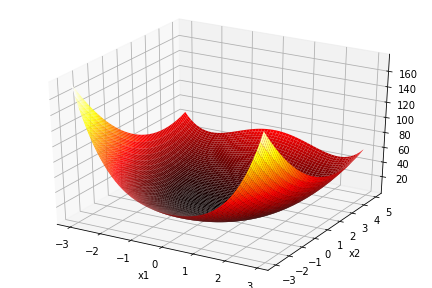
\includegraphics[scale=.6]{function.png}
\caption{函数值关于$x_1$和$x_2$的绘图。}
\label{fig:function}
\end{figure} 

注意到这是一个凸问题,关于局部收敛的讨论是无意义的。在经过简单的尝试后,我们决定设定超参数为$\eta_1=0.1,\;\eta_2=1,\;\kappa_d=10^{-4},\;\kappa_H=1,\;\gamma_d=0.5,\;\gamma_i=1.5,\;\Delta_{max}=10^4,\;\Delta_{min}=10^{-13}$。初始点$x_0$由标准正态分布生成。限制算法至多运行3000个循环。考虑到实验效率,我们也设定中止条件。若$\left|f(x^k)-f(x^{k+1})\right|<conv\_tol=10^{-9}$连续若干个轮次(我们使用的是3个),则代表序列很可能已经收敛,所以算法被中止。我们特别关心每一循环中,用于建立局部无导数模型的点的数量。点的数量很大程度上影响了效率与精度。图\ref{fig:npt}展示了不同点的数量对两者的影响。综合考虑下,我们设定点的数量为10,这一选择能够同时使得模型具有合理的精度和速度。对于大维问题,点的数量应当大于维度,所以点的数量$npt=\max\{10,n\cdot[1+\frac{1}{\log{n}}]\}$。

\begin{figure}[ht!]
    \centering
    \begin{subfigure}{.45\textwidth}
    	\centering
        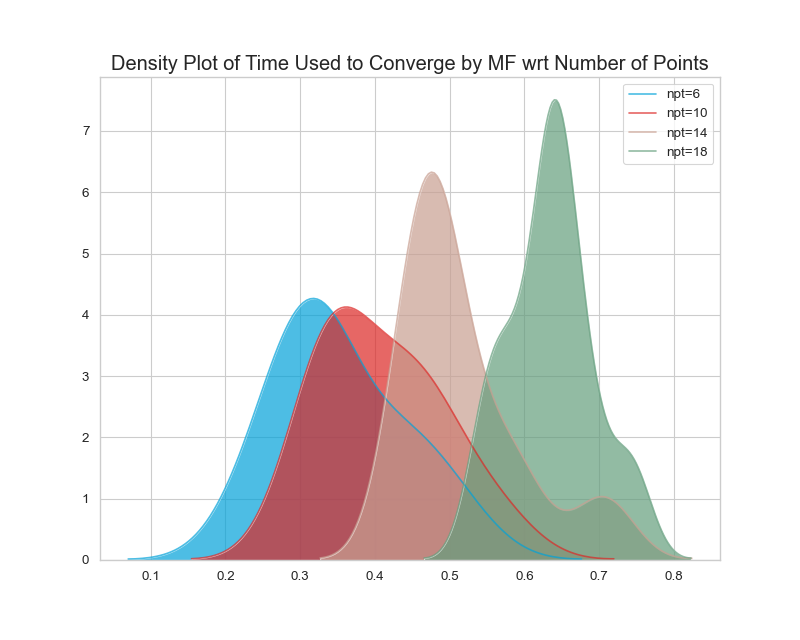
\includegraphics[width=0.9\textwidth]{npttime.png}
    \end{subfigure}
    \begin{subfigure}{.45\textwidth}
    	\centering
        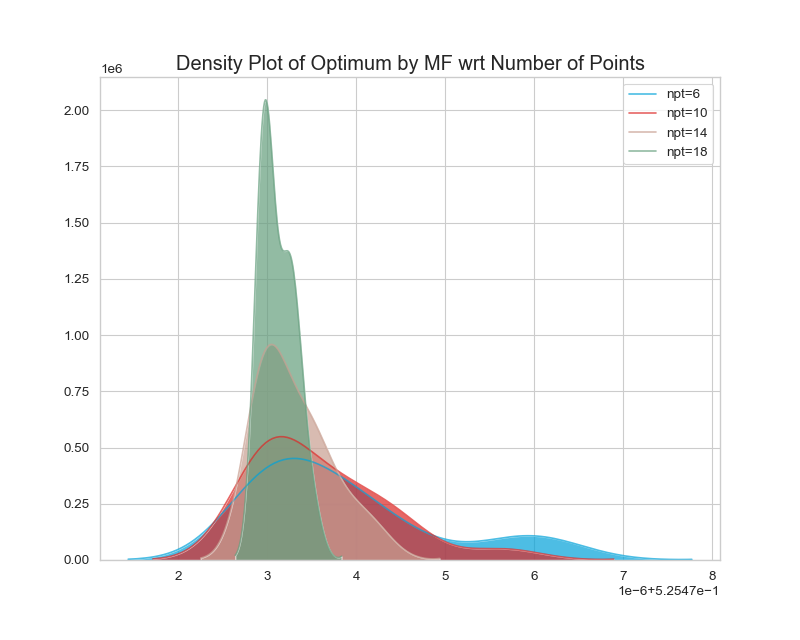
\includegraphics[width=0.9\textwidth]{nptvalue.png}
    \end{subfigure}
    \caption{(彩色模式浏览)时间与函数值关于不同样本点个数的分布。毫无意外的,增加点的个数会使得模型更稳健,同时会增加求解时间。}
\label{fig:npt}
\end{figure}


接下来我们对比流形采样与基准模型。我们选择两个基准模型。第一个是无导数优化模型“Least Square Derivative Free Optimization Tool Box”,由\cite{dfols}开发。选择该模型的目的是比较流形采样与其他无导数优化模型。第二个是基于PyTorch的简单梯度下降。这一方法能够使用的前提是h是分段光滑的,且F(x)落入非光滑的部分的支集为零测集。选取这一基准的目的是为后文结合流形采样与神经网络训练作准备。图\ref{fig:compare}展示了结果对比与流形采样的优越性。

  \begin{figure}[ht!]
    \centering
    \begin{subfigure}{.4\textwidth}
    	\centering
        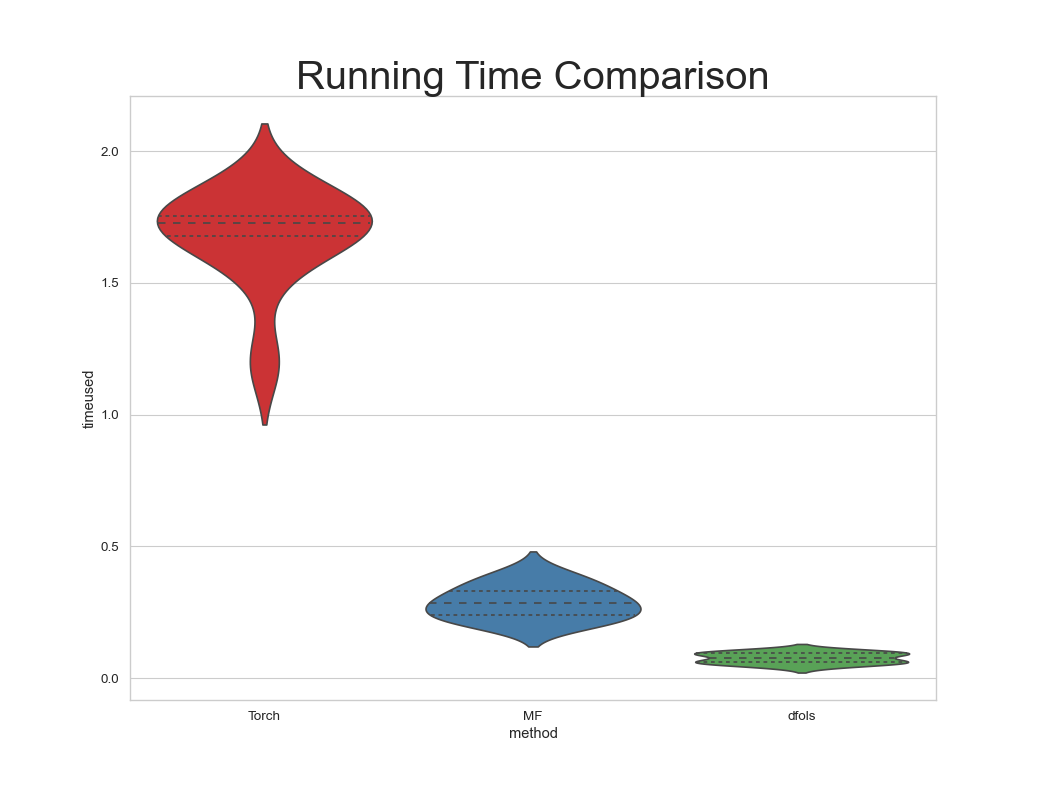
\includegraphics[width=0.9\textwidth]{timecompare.png}
    \end{subfigure}
    \begin{subfigure}{.5\textwidth}
    	\centering
        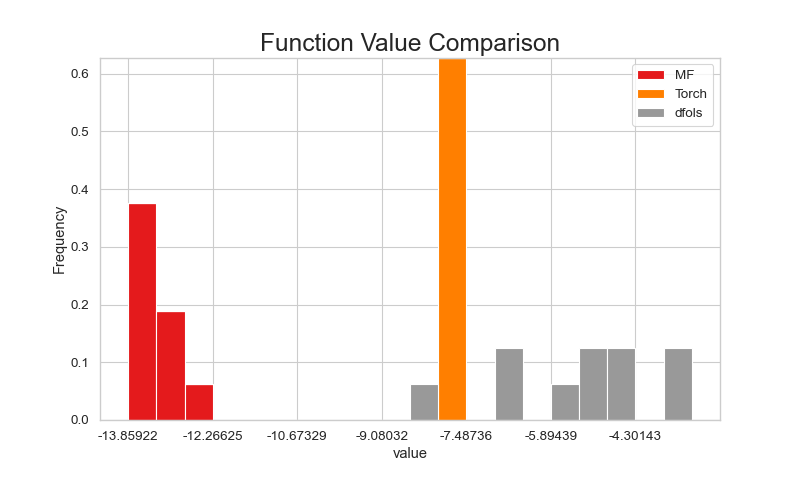
\includegraphics[width=0.9\textwidth]{valuecompare.png}
    \end{subfigure}
    \caption{(彩色模式浏览)三种模型的结果比较。函数值所取的是优化结果与理论最优的差值的log尺度。流形采样得到了最高的精度,同时其运行时间相对较短。}
\label{fig:compare}
\end{figure}
 
 然而,Rosenbrock函数\ref{testfunc1}是非负的,也就是说$L^1$范数失去了意义。我们将问题变为
\begin{equation}
\label{testfunc2}
\phi(x)+h(F(x))=||x||_2+||((x_2-x_1^2)^2-(1-x_1)^2,x_3)||_1,\;x\in \mathbb{R}^3
\end{equation}
这是一个非凸的问题,它在原点附近的行为如图\ref{fig:function2}。

  \begin{figure}[ht!]
    \centering
    \begin{subfigure}{.45\textwidth}
    	\centering
        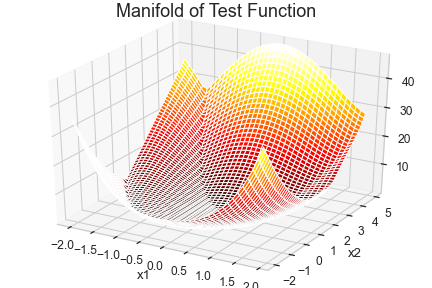
\includegraphics[width=0.9\textwidth]{function2.png}
    \end{subfigure}
    \begin{subfigure}{.45\textwidth}
    	\centering
        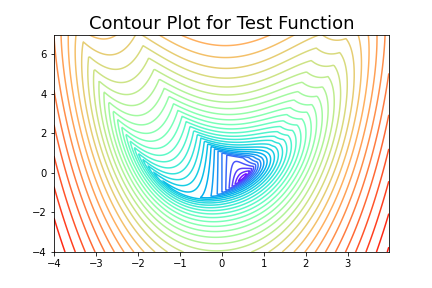
\includegraphics[width=0.9\textwidth]{contour.png}
    \end{subfigure}
    \caption{(彩色模式浏览)测试函数绘图。左图是原点附近的函数曲面,右图为log尺度的函数值等高线图。}
\label{fig:function2}
\end{figure}



算法在这一测试问题上的表现,请查附录\ref{ap2}。


\section{基准测试集}
我们采用\cite{benchmark}作为基准测试集。这一测试集是为了非光滑优化特别设计的,并且可以在任意数据维度下进行测试。测试集的细节,请查附录\ref{ap3}。实验结果在表\ref{tab:result}中进行了展示。需要强调的是,大多数的测试问题原始维度为2,流形采样几乎出色地完成了所有该维度的问题。高维情况的探索实验证明了流形采样能够完成高维的任务,是一类强大的算法。

% Please add the following required packages to your document preamble:
% \usepackage{multirow}
\begin{table}[]
\centering
\caption{基准测试集上的实验结果。我们总共在九个问题上测试了流形采样算法(测试集包含十个问题,然而问题7不符合流形采样要求的问题形式\ref{problem},其非光滑性必须出现在复合的两个阶段)。我们设定自变量的维度为n=2,5,10和100来测试各种维度下的表现。F的像空间维度是自蕴的,我们在\ref{ap3}中展示。为了方便接下来的讨论,我们也列出在最值点某个邻域内$h(L_{\nabla F_i},\cdots)$的上界,记为“曲率”。所有的实验结果记录的均为单次实验值,但每种情况都至少有五次平行实验保障类似结果的获得。收敛指$x^k$和$f(x^k)$是收敛的,到达最值指的是$x^k$和$f(x^k)$收敛到理论最值附近。误差为log尺度的优化结果与理论最优差值。问题"Chained Milfflin"无法获取理论最优,所以收敛时采用柯希极限,不收敛时留白。误差下极限为潜在的收敛做出了提示。时间单位为秒。留白的位置为无意义。}
\begin{tabular}{c|c|ccccccc}
\hline
问题                                                                              & 曲率                 & n   & 收敛 & \begin{tabular}[c]{@{}c@{}}到达 \\ 最值\end{tabular} & 误差 & \begin{tabular}[c]{@{}c@{}}误差 \\ 下极限\end{tabular}  & 时间 & 循环 \\ \hline
\multirow{4}{*}{\begin{tabular}[c]{@{}c@{}}General\\ MAXQ\end{tabular}}   & \multirow{4}{*}{2}        & 2   & Y           & Y                                                        & -9    & -9           & 1.71    & 150       \\ 
                                                                                     &                           & 5   & Y           & Y                                                        & -9    & -9           & 3.59    & 300       \\ 
                                                                                     &                           & 10  & Y           & Y                                                        & -9    & -9           & 6.57    & 500       \\ 
                                                                                     &                           & 100 & Y           & Y                                                        & -5    & -5           & 140     & 3000      \\ \hline
\multirow{4}{*}{\begin{tabular}[c]{@{}c@{}}General\\ MXHILB\end{tabular}} & \multirow{4}{*}{1}        & 2   & Y           & Y                                                        & -6    & -6           & 5.46    & 300       \\  
                                                                                     &                           & 5   & Y           & Y                                                        & -5    & -5           & 51      & 3000      \\  
                                                                                     &                           & 10  & Y           & Y                                                        & -5    & -5           & 107     & 3000      \\  
                                                                                     &                           & 100 & Y           & Y                                                        & -3    & -5           & 5598    & 3000      \\ \hline
\multirow{4}{*}{Chained LQ}                                                          & \multirow{4}{*}{2(n-1)}   & 2   & Y           & Y                                                        & -6    & -6           & 2.74    & 100       \\  
                                                                                     &                           & 5   & Y           & Y                                                        & -3    & -5           & 112     & 3000      \\  
                                                                                     &                           & 10  & Y           & \textit{\textbf{N}}                                      &       & -5           & 180     & 3000      \\  
                                                                                     &                           & 100 & N           & Y                                                        &       & -5           &         &           \\ \hline
\multirow{4}{*}{\begin{tabular}[c]{@{}c@{}}Chained\\ CB3 1\end{tabular}}                                                   & \multirow{4}{*}{12(n-1)}  & 2   & Y           & Y                                                        & -8    & -8           & 21.4    & 1000      \\  
                                                                                     &                           & 5   & Y           & \textit{\textbf{N}}                                      & -1    & -4           & 20.0    & 250       \\  
                                                                                     &                           & 10  & N           & N                                                        &       & -1           &         &           \\  
                                                                                     &                           & 100 & N           & N                                                        &       & -1           &         &           \\ \hline
\multirow{4}{*}{\begin{tabular}[c]{@{}c@{}}Chained \\ CB3 2\end{tabular}}            & \multirow{4}{*}{12}       & 2   & Y           & Y                                                        & -9    & -9           & 27.3    & 1450      \\  
                                                                                     &                           & 5   & Y           & Y                                                        & -3    & -4           & 61.6    & 3000      \\  
                                                                                     &                           & 10  & Y           & Y                                                        & -3    & -3           & 80.4    & 3000      \\  
                                                                                     &                           & 100 & Y           & Y                                                        & -3    & -3           & 590     & 3000      \\ \hline
\multirow{4}{*}{\begin{tabular}[c]{@{}c@{}}Number of \\ Active Faces\end{tabular}}   & \multirow{4}{*}{$\infty$} & 2   & Y           & Y                                                        & -9    & -9           & 3.30    & 130       \\  
                                                                                     &                           & 5   & N           & N                                                        &       & -1           &         &           \\  
                                                                                     &                           & 10  & N           & N                                                        &       & -1           &         &           \\  
                                                                                     &                           & 100 & N           & N                                                        &       & -1           &         &           \\ \hline
\multirow{4}{*}{Chained Milfflin}                                                    & \multirow{4}{*}{2(n-1)}   & 2   & Y           & Y                                                        & -9    & -9           & 31.3    & 1600      \\  
                                                                                     &                           & 5   & Y           & Y                                                        & -6    & -6           & 71.7    & 3000      \\  
                                                                                     &                           & 10  & N           & N                                                        &       &              &         &           \\  
                                                                                     &                           & 100 & N           & N                                                        &       &              &         &           \\ \hline
\multirow{4}{*}{\begin{tabular}[c]{@{}c@{}}Chained\\ Crescent 1\end{tabular}}                                                & \multirow{4}{*}{2}        & 2   & Y           & Y                                                        & -9    & -9           & 3.14    & 150       \\  
                                                                                     &                           & 5   & Y           & Y                                                        & -8    & -8           & 22      & 700       \\  
                                                                                     &                           & 10  & Y           & Y                                                        & -7    & -7           & 30      & 1200      \\  
                                                                                     &                           & 100 & Y           & Y                                                        &       & -3           &   90      &    3000       \\ \hline
\multirow{4}{*}{\begin{tabular}[c]{@{}c@{}}Chained\\ Crescent 2\end{tabular}}                                            & \multirow{4}{*}{2(n-1)}   & 2   & Y           & Y                                                        & -7    & -7           & 2.11    & 150       \\  
                                                                                     &                           & 5   & N           & N                                                        &       & -4           &         &           \\  
                                                                                     &                           & 10  & N           & N                                                        &       & -1           &         &           \\  
                                                                                     &                           & 100 & N           & N                                                        &       & 1            &         &           \\ \hline
\end{tabular}


\label{tab:result}
\end{table}

对所有的测试问题,函数有唯一的全局最优,所以我们期待“收敛”与“到达最值”是等价的。然而,在问题"Chained CB3 1"和"Chained LQ"中,这一推测被推翻了。这并不是偶然的数值爆炸。我们进一步检查了“曲率”这一变量,发现这两个问题中,曲率在最值附近很大。我们将原因归结于该量。

我们注意到在实验中,有些发散序列会存在收敛子列收敛到全局最优。关于这一现象我们有两种猜测,一是数值爆炸,二是函数F本身的性质。我们相信第二个原因占了主导。例如,在误差比较大(或者不收敛)但误差下极限很小的实验中,比如"Chained CB3 1" "Number of Active Faces"和"Chained Crescent 2",曲率分别为$12(n-1),\;\infty$和$2(n-1)$,均随着n的增大而迅速增大,使得曲率对于函数良好性质的限制作废。更多的,从直觉上来讲,即使三个问题均对于n为2收敛,"Chained CB3 1"和"Chained Crescent 2"有更小的曲率,所以在n为5时它们仍然有很小的下极限,而"Number of Active Faces"没有。算法表现对维度的敏感性也被曲率所体现。即使n为100时,"MAXQ", "MXHILB", "CB3 2"和"Crescent 1"仍然有很好的收敛,我们推测这正是因为他们的曲率都相对较小。

\section{非凸性}
我们强调,虽然基准测试集中函数有非凸的性质,但使用的h均为凸函数,无法体现流形采样的独特优越性。我们接下来尝试优化非凸的h。

\begin{equation}
\label{testfunc3}
\phi(x)+h(F(x))=-exp(-||x||^2)+h((x_2-x_1^2)^2,(1-x_1)^2), \;x\in \mathbb{R}^2
\end{equation}
其中
$$
h(z)=\sum_{i=1}^m |1-z_i^2|
$$
函数在零点周围的性质如图\ref{fig:function3}。


    \begin{figure}[ht!]
    \centering
    \begin{subfigure}{.45\textwidth}
    	\centering
        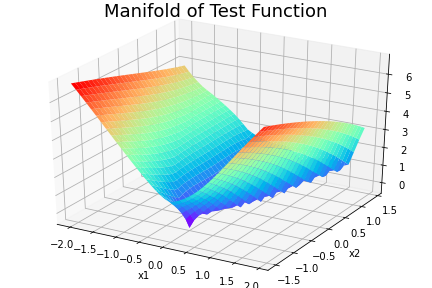
\includegraphics[width=0.9\textwidth]{function3.png}
    \end{subfigure}
    \begin{subfigure}{.45\textwidth}
    	\centering
        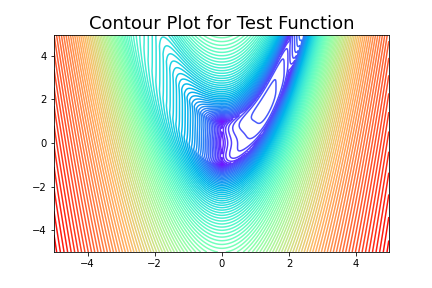
\includegraphics[width=0.9\textwidth]{contourtry.png}
    \end{subfigure}
    \caption{(彩色模式浏览)测试函数绘图。左图是原点附近的函数曲面,右图为log尺度的函数值等高线图。该函数有五个局部极小,(0,0)(0,1)(0,-1)(2,3)(2,5)。}
\label{fig:function3}
\end{figure}

我们以$[-3,3]\times [-3,3]$上的均匀分布生成1000个初始点来测试流形采样算法的局部收敛性。在大多数实验中,序列成功的收敛到附近的极小值,我们在图\ref{fig:convergence}中展示这一结果。由于计算资源的限制,在如此大的样本量下我们无法使用小步长搜索。 
  
  \begin{figure}[H]
\centering

  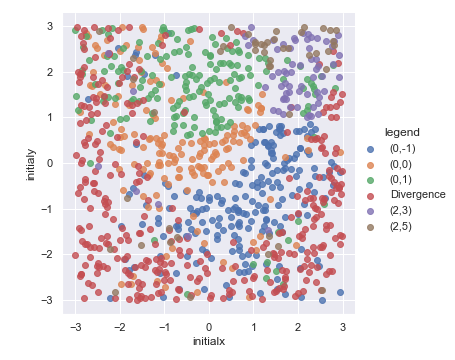
\includegraphics[width=0.8\linewidth]{convergence1.png}

   \caption{(彩色模式浏览)初始值点关于收敛结果的分类图。我们注意到仍有许多发散点。这是由于收到计算资源限制,我们只能选取大步长来进行\ref{minimize},导致$x^k$在两个“斜面”来回跳跃。给予足够的时间,这些点仍然会收敛到局部极小。}
\label{fig:convergence}
  \end{figure}
  

\section{实证研究}

实证研究的部分,我们采用流形采样算法来优化前向神经网络,从而完成回归任务。我们使用\cite{lars}中提供的糖尿病数据集。该数据集总共有十个基本变量,包括年龄、性别、BMI、平均血压和六个血液指标。响应变量是糖尿病一年后病情发展的量化指标。该数据集包括442个样本。我们建立前向神经网络,网络包含一个隐藏层,共10个隐藏单元,采用 sigmoid函数作为激活函数。优化目标是添加了$L^1$惩罚的回归损失
$$
\sum(f(x;w)-y)^2+\lambda||w||_1
$$

考虑到样本量相对较小,我们仅采用梯度下降作为基准,在\ref{fig:loss}中记录两种方法的损失函数随时间的下降。虽然结果并不稳定,但流形采样能够更快的收敛到损失相对小的点。
  
  \begin{figure}[H]
\centering
  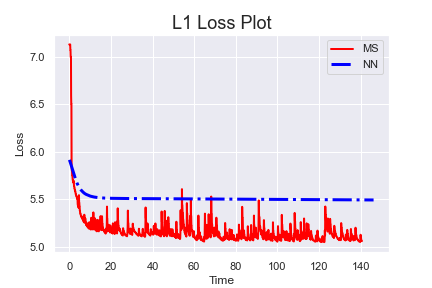
\includegraphics[width=0.8\linewidth]{loss.png}
   \caption{(彩色模式浏览)log尺度损失随着时间的变化。流形采样迅速的下降至小于梯度下降的点。作为相对原始的基准方法,梯度下降没有采用batch norm或者learning rate decay等技巧。相应的,流形采样也没有系统化的调参方法。流形采样损失的震荡可以归结于神经网络损失曲面的高曲率。我们相信,如果存在合理的自动调参方法,损失函数可以稳定的趋于极小。}
\label{fig:loss}
\end{figure}

\chapter{总结与展望}
在本文中,我们拓展已有的流形采样算法至更加广泛的形式,允许f的形式为$f=h\circ F+\phi$,其中$\phi$为光滑函数,使得算法能够对一类常用形式的非光滑、非凸复合函数进行优化。在证明了算法收敛性的同时,我们完成了丰富的数值试验,在标准测试集上检验了算法,讨论了实验结果。最后,我们采用该算法训练浅层神经网络,为未来工作提供可能性。

在后续研究中,我们认为有以下方向值得探索:
\begin{itemize}
\item 对“曲率”与算法是否收敛的关系的探索。我们合理的猜测,在不合适的参数设定下,算法仍然有Minimax收敛,且收敛速率与曲率有关。
\item 自动调参方法。在手动调节参数的过程中,我们能够发现特定参数对于算法行为的影响。比如,$\eta_1$能够控制通过检验的循环质量,从而控制收敛速度与精度的动态平衡。在运行一段时间后,显然我们应当逐渐减小$\eta_1$,以获得更精确的收敛。这启发我们寻找与学习率衰减类似的自动调参方法。
\item 使用算法进行神经网络训练。非光滑正则项,如$L^q,\;0<q<1$,被相信能够为神经网络参数提供更好的惩罚。常见的优化方法并不能很好的处理这类问题。
\end{itemize}



\bibliography{sample}

%%%%%%%%%%%%%%%%%%%%%%%%%%%%%%%%%%%%%%%%%%%%%%%%%%%%%%%%%%%%%%%%%%%%%%%%%%%%%%%
% 致谢,应放在结论之后
\begin{acknowledgement}
感谢帮助我完成这一毕业课题的顾国勇老师,以及和我讨论的两位同学。
感谢南京大学四年来的培养;感谢杜克大学让我度过了精彩的一学期。
感谢南大友鸭,夜间一块肉,快活似神仙。
感谢皇家马德里俱乐部,我会继续买马塞洛的球衣。
感谢宜宾燃面,如果让我选三张照片纪念在南京的日子,我一定和牛杂面自拍一张。不会加磨皮,面会丑。
感谢亚瑟士,让我的脚底得到极致享受。讲实话,落地声音有点大。但这又怎么能怪孩子呢?是我的步子太沉重。
感谢实况足球,没有社交生活的人终于有事情可做。
感谢农夫山泉,让我有水喝。
感谢California Dreaming,在仙二503引吭高歌的时光总是从这首歌开始。但其实,我唱得挺难听的。
感谢莱特币,暴跌时没有带走我,暴涨时却带上了我。
感谢La La Land,在六个没有能量的日子里拉了我一把。很难想象洛杉矶的爱情故事有这样的作用,只能说形成了相当稳定的看电影-变开心的反射过程。
感谢今田美樱,福冈第一美少女的笑永远能让人开心起来,祝新剧大热。
感谢在我生命中出现的每个人,生命因你们而美丽。

\end{acknowledgement}


\appendix
\chapter{材料}
 \section{代码}
 \label{ap1}
 算法的主要伪代码为\ref{algorithm1}。\ref{algorithm2}是\ref{algorithm1}需要调用的函数。

\begin{algorithm}
        \caption{流形采样}
        \label{algorithm1}
        \begin{algorithmic}[1] %每行显示行号
\STATE{Set $\eta_{1}, \kappa_{\mathrm{d}} \in(0,1), \kappa_{\mathrm{H}} \geq 0, \eta_{2} \in\left(0, \eta_{\max }\right), 0<\gamma_{\mathrm{d}}<1 \leq \gamma_{\mathrm{i}}, \text { and } \Delta_{\max }, \Delta_{\min }>0$}
\STATE{Choose $\Delta_0$ in $(0,\Delta_{max}]$ and initialize $x^0$}
		  \FOR{$k= 0 \to K$}
		  \STATE Build master model $m^F$
		  \STATE Initialize $\mathbb{Z}^k$ and Form $D^k$
		  \WHILE{true}
		  \STATE Form $\nabla m^F$
		  \STATE $G^{k} \gets \nabla M\left(x^{k}\right) D^{k}+(\nabla \phi(x^k),\cdots,\nabla \phi(x^k))$
		  \STATE Solve \ref{quadratic} for $\lambda^*$
		  \STATE $d^k\gets D^k \lambda^*$,$g^k\gets G^k\lambda^*$
		  \IF{$\Delta_k<\Delta_{min}$}
		  \STATE Break
		  \ENDIF
		  \IF{$\Delta_k<\eta_2||g^k||$}
		  \STATE Solve \ref{minimize} to get $s^k$
		  \STATE Get z and j satisfying \ref{findz} using Algorithm 2
		  \IF{$j\in \mathbb{A}(\mathbb{Z}^k)$ and no z' satisfies \ref{zprime}}
		  \STATE $s^k\gets -\Delta_{k} \frac{g^{k}}{\left\|g^{k}\right\|}$
		  \STATE Get z and j satisfying \ref{findz} using Algorithm 2
		  \ENDIF
		  \IF{$j\in\mathbb{A}(\mathbb{Z}^k)$}
		  \STATE Calculate $\rho_k$ using \ref{rho},Break
		  \ELSE
		  \STATE Update $m^F$ and $Z\mathbb{Z}^k$,Form $D^k$
		  \ENDIF
		  \ELSE
		  \STATE $\rho_k\gets 0$,Break
		  \ENDIF
		  \ENDWHILE
		  \IF{$\rho_k>\eta_1>0$}
		  \STATE $x^{k+1}\gets x^k+s^k$
		  \STATE $\Delta_{k+1}\gets min\{\gamma_i\Delta_k,\Delta_{max}\}$
		  \ELSE
		  \STATE $x^{k+1}\gets x^k$
		  \STATE {$\Delta_{k+1}\gets \gamma_d\Delta_k$}
		  \ENDIF
		  \ENDFOR
		  
\end{algorithmic}
\end{algorithm}

\newpage
\begin{algorithm}	
	
        \caption{网格搜索求解z与j}
        \label{algorithm2}
        \begin{algorithmic}[1] %每行显示行号
        \IF {$x^z=x$, F(x) and j satisfy \ref{findz}}
        \STATE\RETURN{F(x) and j}
        \ENDIF
        \IF {$x^z=x+s$, F(x+s) and j satisfy \ref{findz}}
        \STATE\RETURN{F(x+s) and j}
        \ENDIF
        \FOR{$l=0,\cdots$}
        \STATE Generate $\{\frac{2 k-1}{2^{l}}: k=1, \ldots, 2^{l-1}\}$
        \FOR{$k=1, 2, \cdots 2^{l-1}$}
        \STATE $\alpha\gets\frac{2k-1}{2^l}$
        \STATE $z(\alpha)\gets\alpha F(x)+(1-\alpha)F(x+s)$
         \IF {$x^z=x+(1-\alpha)s,\; z(\alpha)$ and j satisfy \ref{findz}}
        \STATE\RETURN{$z(\alpha)$and j}
        \ENDIF
        
        \ENDFOR
        \ENDFOR
\end{algorithmic}
\end{algorithm}



 \section{测试结果}
 \label{ap2}
 
我们采取与之前相同的测试方法,结果展示在图 \ref{fig:npt2}与\ref{fig:compare2}中。


    \begin{figure}[ht!]
    \centering
    \begin{subfigure}{.45\textwidth}
    	\centering
        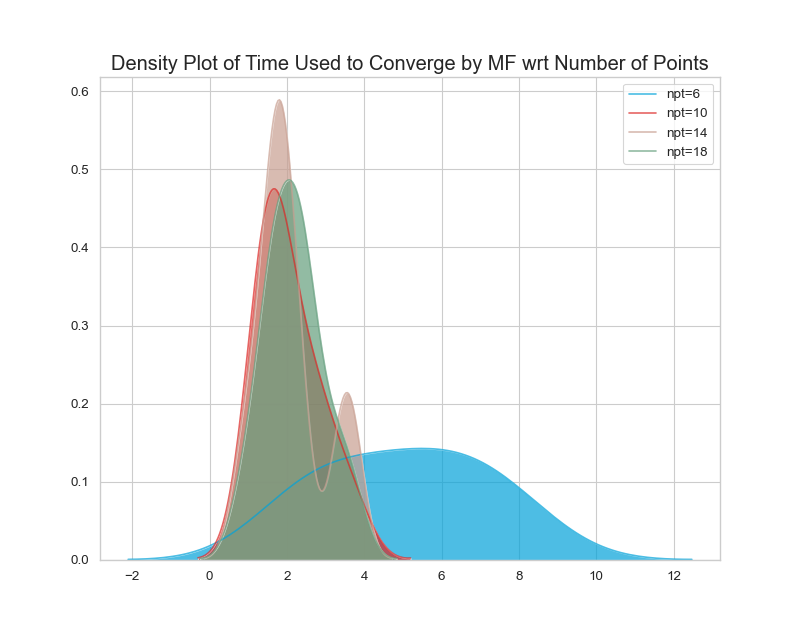
\includegraphics[width=0.9\textwidth]{npttime2.png}
    \end{subfigure}
    \begin{subfigure}{.45\textwidth}
    	\centering
        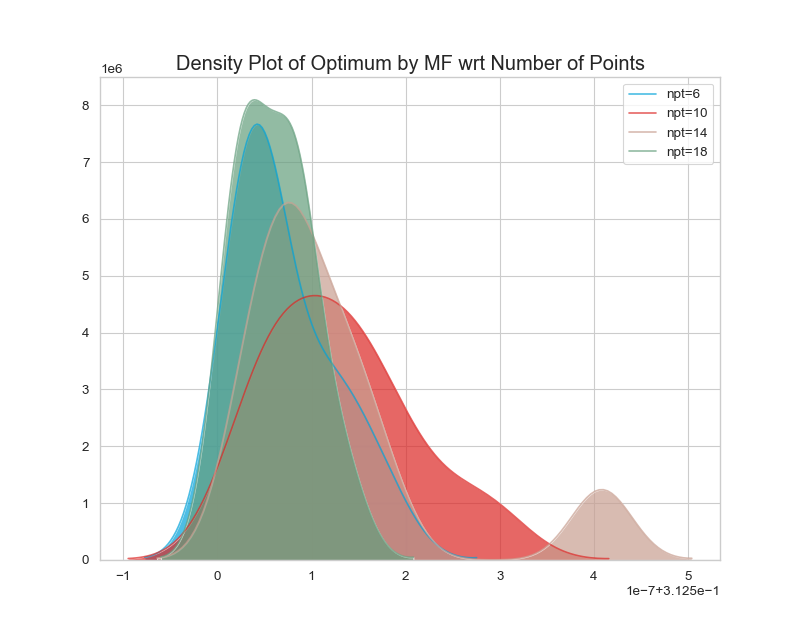
\includegraphics[width=0.9\textwidth]{nptvalue2.png}
    \end{subfigure}
    \caption{(彩色模式浏览)时间与函数值关于不同样本点个数的分布。在样本数为14时有一次实验遭遇了数值爆炸,所以该类别表现很差。}
\label{fig:npt2}
\end{figure}

  \begin{figure}[ht!]
    \centering
    \begin{subfigure}{.4\textwidth}
    	\centering
        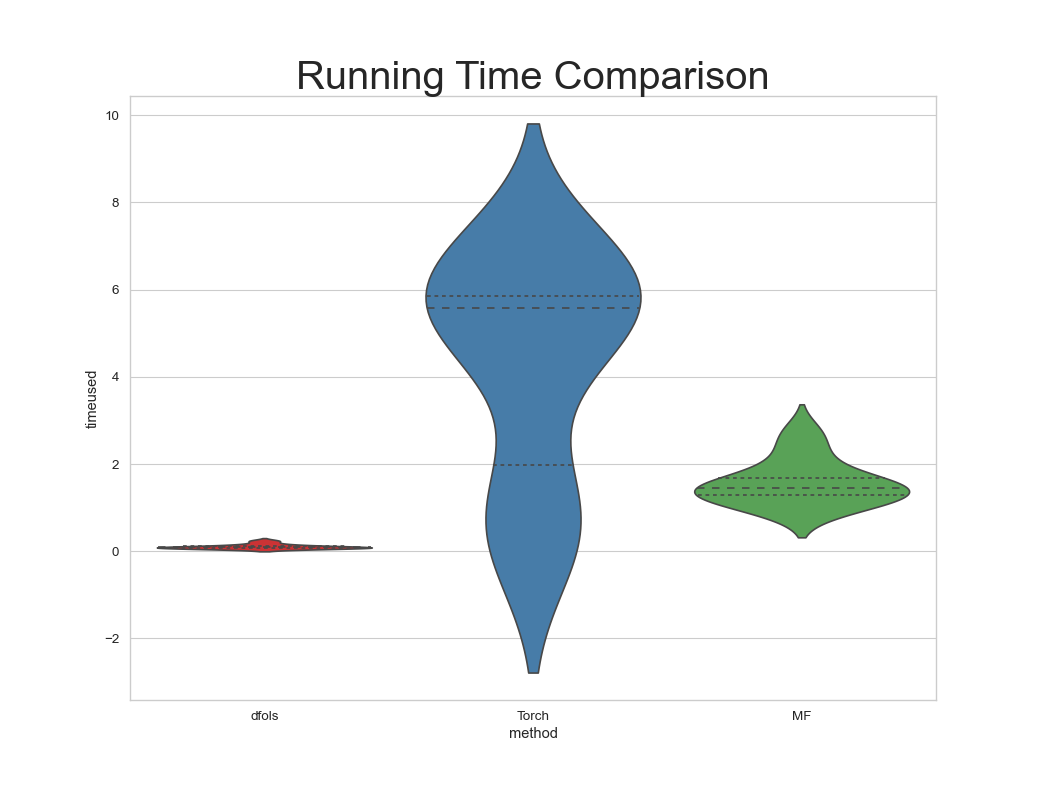
\includegraphics[width=0.9\textwidth]{timecompare2.png}
    \end{subfigure}
    \begin{subfigure}{.5\textwidth}
    	\centering
        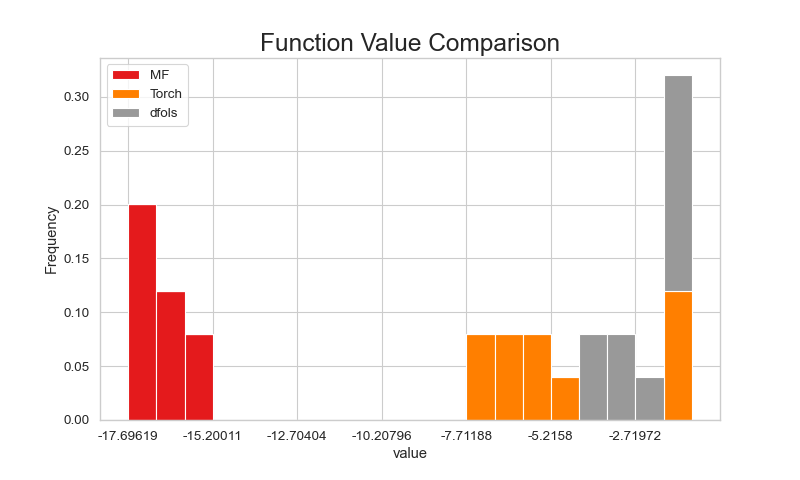
\includegraphics[width=0.9\textwidth]{valuecompare2.png}
    \end{subfigure}
    \caption{(彩色模式浏览)三种模型的结果比较。函数值所取的是优化结果与理论最优的差值的log尺度。流形采样得到了最高的精度,同时其运行时间相对较短。}
\label{fig:compare2}
\end{figure}







 \section{基准数据集}
 \label{ap3}
 我们提供\cite{benchmark}的细节。
 \begin{enumerate}
 
 \item Generalization of MAXQ
 \begin{flalign}
 \hspace{3mm}&
 \begin{array}{l}
f(\mathbf{x})=\max _{1 \leq i \leq n} x_{i}^{2} \\
x_{i}^{(1)}=i, \quad \text { for } i=1, \ldots, n / 2 \text { and } \\
x_{i}^{(1)}=-i, \quad \text { for } i=n / 2+1, \ldots, n .
\end{array}
&
\nonumber
\end{flalign}

 \item Generalization of MXHILB
 \begin{flalign}
 \hspace{3mm}&
\begin{array}{l}
f(\mathbf{x})=\max _{1 \leq i \leq n}\left|\sum_{j=1}^{n} \frac{x_{j}}{i+j-1}\right| \\
x_{i}^{(1)}=1, \quad \text { for all } i=1, \ldots, n
\end{array}
&
\nonumber
\end{flalign}

 \item Chained LQ
 \begin{flalign}
 \hspace{3mm}&
\begin{array}{l}
f(\mathbf{x})=\sum_{i=1}^{n-1} \max \left\{-x_{i}-x_{i+1},-x_{i}-x_{i+1}+\left(x_{i}^{2}+x_{i+1}^{2}-1\right)\right\} \\
x_{i}^{(1)}=-0.5, \text { for all } i=1, \ldots, n
\end{array}
&
\nonumber
\end{flalign}

 \item Chained CB3 1
 \begin{flalign}
 \hspace{3mm}&
\begin{array}{l}
f(\mathbf{x})=\sum_{i=1}^{n-1} \max \left\{x_{i}^{4}+x_{i+1}^{2},\left(2-x_{i}\right)^{2}+\left(2-x_{i+1}\right)^{2}, 2 e^{-x_{i}+x_{i+1}}\right\} \\
x_{i}^{(1)}=2, \quad \text { for all } i=1, \ldots, n
\end{array}
&
\nonumber
\end{flalign}

 \item Chained CB3 2
 \begin{flalign}
 \hspace{3mm}&
\begin{array}{l}
f(\mathbf{x})=\max \left\{\sum_{i=1}^{n-1}\left(x_{i}^{4}+x_{i+1}^{2}\right), \sum_{i=1}^{n-1}\left(\left(2-x_{i}\right)^{2}+\left(2-x_{i+1}\right)^{2}\right)\right. \\
\left.\sum_{i=1}^{n-1}\left(2 e^{-x_{i}+x_{i+1}}\right)\right\} \\
x_{i}^{(1)}=2, \quad \text { for all } i=1, \ldots, n
\end{array}
&
\nonumber
\end{flalign}

 \item Number of Active Faces
 \begin{flalign}
 \hspace{3mm}&
\begin{array}{l}
f(\mathbf{x})=\max _{1 \leq i \leq n}\left\{g\left(-\sum_{i=1}^{n} x_{i}\right), g\left(x_{i}\right)\right\} \\
\text { where } g(y)=\ln (|y|+1) \\
x_{i}^{(1)}=1, \quad \text { for all } i=1, \ldots, n
\end{array}
&
\nonumber
\end{flalign}

 \item Chained Mifflin
 \begin{flalign}
 \hspace{3mm}&
\begin{array}{l}
f(\mathbf{x})=\sum_{i=1}^{n-1}\left(-x_{i}+2\left(x_{i}^{2}+x_{i+1}^{2}-1\right)+1.75\left|x_{i}^{2}+x_{i+1}^{2}-1\right|\right) \\
x_{i}^{(1)}=-1, \quad \text { for all } i=1, \ldots, n
\end{array}
&
\nonumber
\end{flalign}

 \item Chained Crescent 1
 \begin{flalign}
 \hspace{3mm}&
\begin{aligned}
&\begin{array}{r}
f(\mathbf{x})=\max \left\{\sum_{i=1}^{n-1}\left(x_{i}^{2}+\left(x_{i+1}-1\right)^{2}+x_{i+1}-1\right)\right. \\
\left.\sum_{i=1}^{n-1}\left(-x_{i}^{2}-\left(x_{i+1}-1\right)^{2}+x_{i+1}+1\right)\right\}
\end{array}\\
&x_{i}^{(1)}=-1.5, \text { when } \bmod (i, 2)=1,(i=1, \ldots, n) \text { and }\\
&x_{i}^{(1)}=2.0, \quad \text { when } \quad \bmod (i, 2)=0,(i=1, \ldots, n) .
\end{aligned}
&
\nonumber
\end{flalign}

 \item Chained Crescent 2
 \begin{flalign}
 \hspace{3mm}&
\begin{aligned}
&\begin{aligned}
f(\mathbf{x})=\sum_{i=1}^{n-1} & \max \left\{x_{i}^{2}+\left(x_{i+1}-1\right)^{2}+x_{i+1}-1,
-x_{i}^{2}-\left(x_{i+1}-1\right)^{2}+x_{i+1}+1\right\} &
\end{aligned}\\
&x_{i}^{(1)}=-1.5, \text { when } \bmod (i, 2)=1,(i=1, \ldots, n) \text { and }\\
&x_{i}^{(1)}=2.0, \quad \text { when } \quad \bmod (i, 2)=0,(i=1, \ldots, n) .
\end{aligned}
&
\nonumber
\end{flalign}


 \end{enumerate}
 
 注意到问题6其实是不符合要求的,因为其不满足全线性\ref{secondlip},但我们仍然保留。表\ref{tab:test}给出了问题的性质。
 
 
 % Please add the following required packages to your document preamble:
% \usepackage{multirow}
\begin{table}[]
\centering
\caption{问题集的性质}
\label{tab:test}
\begin{tabular}{cccccc}
\hline
序号                  & 最小值         & 凸性      & 非光滑函数(h)                                   & $L_h$                                       & m          \\ \hline
\multicolumn{1}{c|}{1} & 0                     & Y              & \multicolumn{1}{c|}{$max(\cdot)$}                   & \multicolumn{1}{c|}{\multirow{9}{*}{1}}     & n          \\ \cline{1-4} \cline{6-6} 
\multicolumn{1}{c|}{2} & 0                     & Y              & \multicolumn{1}{c|}{$max(\left |\cdot\right|)$}     & \multicolumn{1}{c|}{}                       & n          \\ \cline{1-4} \cline{6-6} 
\multicolumn{1}{c|}{3} & $-(n-1)\sqrt{2}$      & Y              & \multicolumn{1}{c|}{$\sum max(\cdot)$}              & \multicolumn{1}{c|}{}                       & 2(n-1)     \\ \cline{1-4} \cline{6-6} 
\multicolumn{1}{c|}{4} & 2(n-1)                & Y              & \multicolumn{1}{c|}{$\sum max(\cdot)$}              & \multicolumn{1}{c|}{}                       & 3(n-1)     \\ \cline{1-4} \cline{6-6} 
\multicolumn{1}{c|}{5} & 2(n-1)                & Y              & \multicolumn{1}{c|}{$max(\cdot)$}                   & \multicolumn{1}{c|}{}                       & 3          \\ \cline{1-4} \cline{6-6} 
\multicolumn{1}{c|}{6} & 0                     & N              & \multicolumn{1}{c|}{$max(\cdot)$}                   & \multicolumn{1}{c|}{}                       & n+1        \\ \cline{1-4} \cline{6-6} 
\multicolumn{1}{c|}{7} & Varies*               & N              & \multicolumn{1}{c|}{$\left|\cdot\right|$}           & \multicolumn{1}{c|}{}                       & n-1        \\ \cline{1-4} \cline{6-6} 
\multicolumn{1}{c|}{8} & 0                     & N              & \multicolumn{1}{c|}{$max(\cdot)$}                   & \multicolumn{1}{c|}{}                       & 2          \\ \cline{1-4} \cline{6-6} 
\multicolumn{1}{c|}{9} & 0                     & N              & \multicolumn{1}{c|}{$\sum max(\cdot)$}              & \multicolumn{1}{c|}{}                       & 2(n-1)     \\ \hline
                       & \multicolumn{5}{c}{\begin{tabular}[c]{@{}c@{}}* n=10时最小值约-6.51\\n=100时约为-70.15,n=1000时约为-706.55\end{tabular}} \\ \hline
\end{tabular}
\end{table}
















%%%%%%%%%%%%%%%%%%%%%%%%%%%%%%%%%%%%%%%%%%%%%%%%%%%%%%%%%%%%%%%%%%%%%%%%%%%%%%%
\end{document}
